\section{Methods}
\subsection{Parallel ideas}

there are several ways to exploit parallelization in the Monte Carlo simulation:

\begin{description}

  \item[samplepoints] ($\rightarrow$ implemented as multiGPU)

    The samples from \ref{label:meshSampling} are independent from each other
    and can therefore be calculated in parallel

  \item[rays] ($\rightarrow$ implented through threads/blocks)
    
    Every ray can be calculated independently from each other.
    Exploiting this parallelism provides a great opportunity to boost
    performance. Only the resulting gains for each sample point have to be
    combined in the end.

  \item[wavelengths]

    According to \label{label:monteCarlo}, the simulation of a polychromatic
    laser can be split into sufficiently small monochromatic simulations which
    are again completely independent from each other.

\end{description}


\subsection{Importance sampling}
\begin{itemize}
\item Importance sampling is a well known technique in the domain
  of statistics \cite{importanceSampling}. In case of ASE-Flux calculation a presampling of
  a sample point is done to figure out important areas
  inside the mesh. Important areas generate more rays for a
  particular sample point.
\item Importance sampling can increase the efficiency of Monte-Carlo-Simulations (reduce variance)
\end{itemize}

\subsection{Adaptive rays}
Since most sample points behave in a good way, they don't need
to be samlped with a high number of rays. Only some outliers need to
be simulated with a higher precision. You can quantify the precision
and therefore the difference between the true and calculated value by
the mean squared error (MSE).
The adaptive method allows you to remove strong peaks in the result
of monte carlo simulation without sampling all sample points with
a high number of rays.
\begin{itemize}
\item MSE: 
     \[f(\vec{r_0}) = \frac{1}{n} \sum_{i=1}^n g_i \]
     \[f^2(r_0) = \frac{1}{n} \sum_{i=1}^n g_i^2 \]
     \[MSE(r_0) = \sqrt{\frac{f^2(r_0) - f(r_0)^2}{n}}\]
\item Dependant on a $MSE$-threshold and the $MSE$ value
  of the sample, the number of rays per sample point 
  will be increased to a maximum number.
\item Thus not every sample point needs to be sampled
  with a high number of rays to obtain high precision.
  Only sample points with $MSE(r_0) \quad \textgreater \quad MSE$-threshold need
  resampling. This saves a lot of calculation time.
\item By decresing the MSE threshold (increasing precision), the runtime increses because
  of a higher number of rays per sample point. It could also happen, that the maximum number
  of rays are not enough to reach the given MSE threshold.
\end{itemize}
\begin{center}
  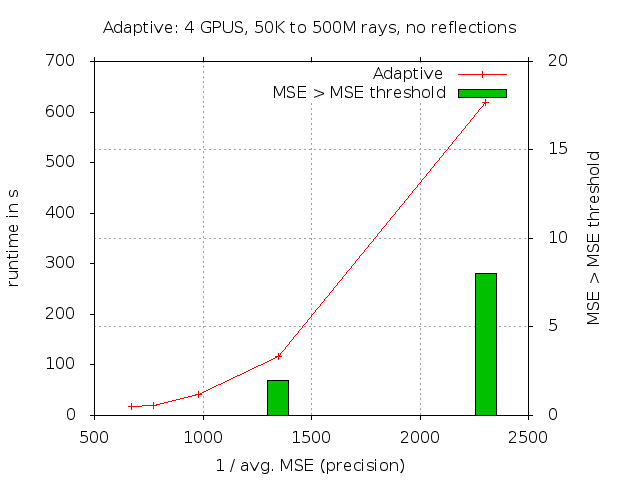
\includegraphics[width=8cm]{plot/adaptive.png}
\end{center}
